스택, 큐, 덱은 데이터의 양 끝에서 연산이 이루어지는 선형 자료구조라는 공통된 특징이 있다. 이 자료구조들은 양 끝에서의 연산만이 요구되는 상황에서 장점을 갖는다. 이번 장에서는 스택, 큐, 덱이 지원하는 연산들을 알아보고, 각각이 어떤 문제에 적합한지 알아볼 것이다.

\section{스택}
스택(stack)은 이름에서도 드러나지만 데이터를 쌓아가는 구조를 가진다. 데이터를 쌓아가는 구조를 만드려면 어떤 연산을 지원해야 할까? 제일 위의 데이터 참조, 데이터를 위에 추가, 제일 위의 데이터 제거의 세 가지 연산만 제공하면 충분할 것이다.

\begin{figure}[htbp]
    \centering
    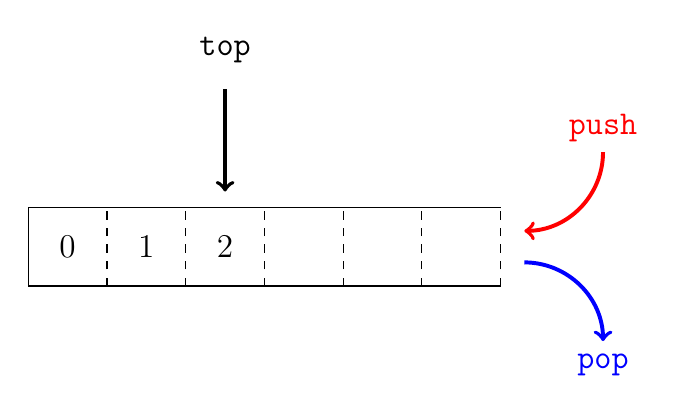
\begin{tikzpicture}
        \draw[-] (0,0) -- (0,1);
        \draw[-] (0,0) -- (6,0);
        \draw[-] (0,1) -- (6,1);
        \draw[dashed] (1,0) -- (1,1);
        \draw[dashed] (2,0) -- (2,1);
        \draw[dashed] (3,0) -- (3,1);
        \draw[dashed] (4,0) -- (4,1);
        \draw[dashed] (5,0) -- (5,1);
        \draw[dashed] (6,0) -- (6,1);
        
        \node[font=\large] at (0.5,0.5) {0};
        \node[font=\large] at (1.5,0.5) {1};
        \node[font=\large] at (2.5,0.5) {2};
        \draw[->, line width=0.5mm] (2.5,2.5) -- (2.5,1.2);
        \node[font=\large] at (2.5,3.0) {\texttt{top}};

        \draw[->, red, line width=0.5mm] (7.3,1.7) arc[start angle=0, end angle=-90, radius=1cm];
        \node[red, font=\large] at (7.3,2.0) {\texttt{push}};
        \draw[<-, blue, line width=0.5mm] (7.3,-0.7) arc[start angle=0, end angle=90, radius=1cm];
        \node[blue, font=\large] at (7.3,-1.0) {\texttt{pop}};
    \end{tikzpicture}
\end{figure}

즉, 스택에서는 제일 위의 데이터가 굉장히 중요하다. 그래서 제일 위의 데이터를 \texttt{top}이라고 한다. \texttt{top}이라는 용어를 이용해서 다시 표현하면, 스택은 \texttt{top}의 값 가져오기, \texttt{top} 위에 새로운 데이터를 쌓기, \texttt{top} 제거하기의 세 가지 연산이 가능하다고 말할 수 있겠다. 그리고 이 모든 연산은 $O(1)$의 시간에 가능하다.

이처럼 제일 나중에 들어온 데이터가 제일 먼저 나가는 구조를 LIFO(last-in-first-out) 구조라고 부른다. 이러한 장점은 \textbf{나중의 것을 먼저 처리}해야만 하는 모든 문제에 적용될 수 있다. 나중에 호출된 함수의 작업이 끝나야 그 전에 호출된 함수를 실행하는 재귀함수나, 나중에 작성한 텍스트부터 지워야 하는 되돌리기(undo) 기능 등을 예시로 들 수 있다.

STL에는 스택이 있다. \url{https://en.cppreference.com/w/cpp/container/stack}에 가면 어떤 함수를 지원하고 어떻게 사용하는지, 시간복잡도까지 모두 확인할 수 있다. 다음은 대표적으로 사용되는 함수들이다.

\begin{itemize}
    \item \texttt{top()}를 통해 제일 위(앞)의 값을 참조할 수 있다.
    \item \texttt{push(T)}를 통해 제일 위(앞)에 값을 추가할 수 있다.
    \item \texttt{pop()}를 통해 제일 위(앞)의 값을 제거할 수 있다.
    \item \texttt{empty()}를 통해 비어있는지 여부를 확인할 수 있다.
    \item \texttt{size()}를 통해 저장된 데이터의 개수를 확인할 수 있다.
\end{itemize}

실제로 STL의 스택을 사용하여 다음의 대표적인 스택 활용 문제를 해결해보자.

\begin{example} \label{ex: stack}
    (9012번) `('와 `)'만으로 이루어진 문자열을 \textbf{괄호 문자열}이라 하자. \textbf{올바른 괄호 문자열}은 다음 세 조건 중 하나 이상을 만족해야 한다.
    \begin{itemize}
        \item 문자열 `()'이거나,
        \item 올바른 괄호 문자열 $S$에 대해 ($S$)이거나,
        \item 올바른 괄호 문자열 $S$와 $T$에 대해 $ST$이다.
    \end{itemize}
    주어진 문자열이 올바른 괄호 문자열인지 판별하라.
\end{example}

이 문제는 왜 스택으로 해결할 수 있을까? 다음의 관찰을 생각해보자.

\begin{obs}
    괄호 문자열은 바깥 괄호쌍 안에 안쪽 괄호쌍이 규칙에 맞게 있어야 한다. 즉, \textbf{나중에} 나온 열린 괄호부터 닫힌 괄호와 매칭해줘야 한다. 이는 스택의 장점인 \textbf{나중에} 것을 먼저 처리하는 것으로 해결할 수 있다. 따라서 스택은 이 문제에 적절한 자료구조이다.    
\end{obs}

위의 사고 과정을 다시 되짚어보자. 우리는 문제를 보고 문제의 해결을 위한 알고리즘인 `나중에 ... 매칭해줘야 한다'를 고안했다. 그리고, 알고리즘의 요구사항인 `나중에'에 장점이 있는 자료구조인 스택을 떠올리고, 스택으로 문제를 해결할 수 있음을 알게 된 것이다.

다시 한번 말하지만, 자료구조는 \textbf{빠르게 할 수 있는 연산}과 같다. 따라서, 자료구조를 쓸 수 있는지 확인하려면, \underline{자료구조의 장점} -- 어떤 연산을 빠르게 할 수 있는가 -- 과 \underline{알고리즘의 요구사항}이 일치하는지 확인하면 된다.

이제 관찰을 바탕으로 실제로 구현을 해보자. \Cref{code: bracket-matching}을 보자.

\begin{code} \label{code: bracket-matching}
\Cref{ex: stack}을 해결하는 코드
\begin{lstlisting}
#include <bits/stdc++.h>
using namespace std;

void solve(string s) {
    stack<int> stk;
    for (int i = 0; i < s.length(); i++) {
        if (s[i] == '(') stk.push('(');
        else {
            if (stk.size() == 0) {
                cout << "NO\n";
                return;
            }
            else stk.pop();
        }
    }
    if (stk.size() == 0) cout << "YES\n";
    else cout << "NO\n";
}

int main() {
    ios_base::sync_with_stdio(false);
    cin.tie(0);
    
    int t;
    cin >> t;
    while (t--) {
        string s;
        cin >> s;
        solve(s);
    }
}
\end{lstlisting}
\end{code}

\section{큐}
큐(queue)은 이름에서도 드러나지만 대기열과 비슷한 구조를 가진다. 대기열과 비슷한 구조를 만드려면 어떤 연산을 지원해야 할까? 제일 앞의 데이터 참조, 데이터를 뒤에 추가, 제일 앞의 데이터 제거의 세 가지 연산만 제공하면 충분할 것이다.

\begin{figure}[htbp]
    \centering
    \begin{tikzpicture}
        \draw[dashed] (0,0) -- (0,1);
        \draw[-] (0,0) -- (6,0);
        \draw[-] (0,1) -- (6,1);
        \draw[dashed] (1,0) -- (1,1);
        \draw[dashed] (2,0) -- (2,1);
        \draw[dashed] (3,0) -- (3,1);
        \draw[dashed] (4,0) -- (4,1);
        \draw[dashed] (5,0) -- (5,1);
        \draw[dashed] (6,0) -- (6,1);
        
        \node[font=\large] at (0.5,0.5) {0};
        \node[font=\large] at (1.5,0.5) {1};
        \node[font=\large] at (2.5,0.5) {2};
        \draw[->, line width=0.5mm] (0.5,2.5) -- (0.5,1.2);
        \node[font=\large] at (0.5,3.0) {\texttt{front}};

        \draw[->, red, line width=0.5mm] (7.3,1.7) arc[start angle=0, end angle=-90, radius=1cm];
        \node[red, font=\large] at (7.3,2.0) {\texttt{push}};
        \draw[<-, blue, line width=0.5mm] (-1.3,-0.7) arc[start angle=180, end angle=90, radius=1cm];
        \node[blue, font=\large] at (-1.3,-1.0) {\texttt{pop}};
    \end{tikzpicture}
\end{figure}

즉, 큐에서는 제일 앞의 데이터가 굉장히 중요하다. 그래서 제일 앞의 데이터를 \texttt{front}라고 한다. 또, 제일 뒤의 데이터를 \texttt{back}이라고 한다. \texttt{front}와 \texttt{back}이라는 용어를 이용해서 다시 표현하면, 스택은 \texttt{front}의 값 가져오기, \texttt{back} 뒤에 새로운 데이터를 추가하기, \texttt{front} 제거하기의 세 가지 연산이 가능하다고 말할 수 있겠다. 그리고 이 모든 연산은 $O(1)$의 시간에 가능하다.

이처럼 제일 먼저 들어온 데이터가 제일 먼저 나가는 구조를 FIFO(first-in-first-out) 구조라고 부른다. 이러한 장점은 \textbf{이른 것을 먼저 처리}해야만 하는 모든 문제에 적용될 수 있다. 선착순으로 입장하는 대기열(하드웨어에서는 프로세스 스케쥴링)이나 BFS(링크) 등을 예시로 들 수 있다.

STL은 큐도 지원한다. \url{https://en.cppreference.com/w/cpp/container/queue}에 가면 어떤 함수를 지원하고 어떻게 사용하는지, 시간복잡도까지 모두 확인할 수 있다. 다음은 대표적으로 사용되는 함수들이다.

\begin{itemize}
    \item \texttt{front()}를 통해 제일 앞의 노드를 참조할 수 있다.
    \item \texttt{back()}를 통해 제일 뒤의 노드를 참조할 수 있다.
    \item \texttt{push(T)}를 통해 제일 뒤에 값을 추가할 수 있다.
    \item \texttt{pop()}를 통해 제일 앞의 값을 제거할 수 있다.
    \item \texttt{empty()}를 통해 비어있는지 여부를 확인할 수 있다.
    \item \texttt{size()}를 통해 저장된 데이터의 개수를 확인할 수 있다.
\end{itemize}

실제로 STL의 큐를 사용하여 다음의 대표적인 큐 활용 문제를 해결해보자.

\begin{example} \label{ex: queue}
    (1158번) $1$번부터 $N$번까지의 사람이 시계방향으로 둘러앉아 있다. 주어진 양의 정수 $K$에 대해 모두가 제거될 때까지 시계방향으로 이동하며 $K$번째 사람을 제거한다. 제거되는 사람의 번호를 순서대로 출력하라.
\end{example}

이 문제는 왜 큐로 해결할 수 있을까? 다음의 관찰을 생각해보자.

\begin{obs}
    내가 가만히 있고, $N$명의 사람들이 움직인다고 생각해보자. 사람들은 한 줄로 서 있고, $K$번째 사람을 만나기 전까지 사람을 줄의 제일 뒤로 보내고, $K$번째 사람을 만나면 그 사람을 죽일 것이다. 즉, 대기열과 비슷한 알고리즘을 해결할 수 있으므로, 큐는 이 문제에 적합한 자료구조이다.
\end{obs}

이제 관찰을 바탕으로 실제로 구현을 해보자. \Cref{code: Josephus}을 보자.

\begin{code} \label{code: Josephus}
\Cref{ex: queue}을 해결하는 코드
\begin{lstlisting}
#include <bits/stdc++.h>
using namespace std;

int main() {
    ios_base::sync_with_stdio(false);
    cin.tie(0);
    
    int n, k;
    cin >> n >> k;
    queue<int> q;

    for (int i = 1; i <= n; i++) q.push(i);
    
    while (!q.empty()) {
        for (int i = 1; i < k; i++) {
            q.push(q.front());
            q.pop();
        }
        cout << q.front();
        q.pop();
    }
    
    return 0;
}
\end{lstlisting}
\end{code}

\section{덱}
덱(deque)은 double-ended queue의 약자로, 큐와 비슷하지만 양쪽 모두에서 \texttt{push}와 \texttt{pop}이 가능한 자료구조이다.

\begin{figure}[htbp]
    \centering
    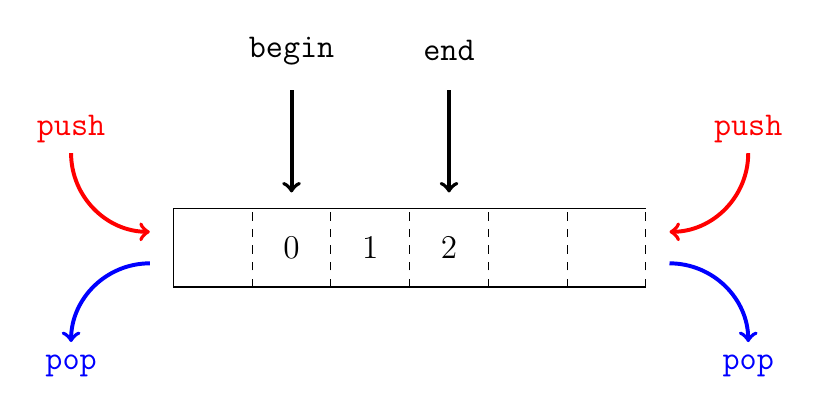
\begin{tikzpicture}
        \draw[-] (0,0) -- (0,1);
        \draw[-] (0,0) -- (6,0);
        \draw[-] (0,1) -- (6,1);
        \draw[dashed] (1,0) -- (1,1);
        \draw[dashed] (2,0) -- (2,1);
        \draw[dashed] (3,0) -- (3,1);
        \draw[dashed] (4,0) -- (4,1);
        \draw[dashed] (5,0) -- (5,1);
        \draw[dashed] (6,0) -- (6,1);
        
        \node[font=\large] at (1.5,0.5) {0};
        \node[font=\large] at (2.5,0.5) {1};
        \node[font=\large] at (3.5,0.5) {2};
        \draw[->, line width=0.5mm] (1.5,2.5) -- (1.5,1.2);
        \node[font=\large] at (1.5,3.0) {\texttt{begin}};
        \draw[->, line width=0.5mm] (3.5,2.5) -- (3.5,1.2);
        \node[font=\large] at (3.5,3.0) {\texttt{end}};

        \draw[->, red, line width=0.5mm] (7.3,1.7) arc[start angle=0, end angle=-90, radius=1cm];
        \node[red, font=\large] at (7.3,2.0) {\texttt{push}};
        \draw[->, red, line width=0.5mm] (-1.3,1.7) arc[start angle=180, end angle=270, radius=1cm];
        \node[red, font=\large] at (-1.3,2.0) {\texttt{push}};
        \draw[<-, blue, line width=0.5mm] (7.3,-0.7) arc[start angle=0, end angle=90, radius=1cm];
        \node[blue, font=\large] at (7.3,-1.0) {\texttt{pop}};
        \draw[<-, blue, line width=0.5mm] (-1.3,-0.7) arc[start angle=180, end angle=90, radius=1cm];
        \node[blue, font=\large] at (-1.3,-1.0) {\texttt{pop}};
    \end{tikzpicture}
\end{figure}

덱은 \texttt{vector}와 유시하게 제일 앞의 데이터를 \texttt{front}라고 한다. 또, 제일 뒤의 데이터를 \texttt{back}이라고 한다. \texttt{front}와 \texttt{back}이라는 용어를 이용해서 다시 표현하면, 스택은 \texttt{front}의 값 가져오기, \texttt{back} 뒤에 새로운 데이터를 추가하기, \texttt{front} 제거하기의 세 가지 연산이 가능하다고 말할 수 있겠다. 그리고 이 모든 연산은 $O(1)$의 시간에 가능하다.

즉, 덱은 스택과 큐의 기능을 모두 지원하는 큰 범주의 자료구조라고 할 수 있겠다. 하지만, 그렇다고 항상 덱을 쓰는 것은 좋은 습관이 아니다. 스택이나 큐만의 연산만을 사용해도 충분한 경우, 스택이나 큐를 사용하는 것이 더 빠를 뿐만 아니라 코드의 가독성이나 알고리즘의 명확성 측면에서 도움이 된다.

STL은 덱도 지원한다. \url{https://en.cppreference.com/w/cpp/container/deque}에 가면 어떤 함수를 지원하고 어떻게 사용하는지, 시간복잡도까지 모두 확인할 수 있다. 다음은 대표적으로 사용되는 함수들이다.

\begin{itemize}
    \item \texttt{front()}를 통해 제일 앞의 노드를 참조할 수 있다.
    \item \texttt{back()}를 통해 제일 뒤의 노드를 참조할 수 있다.
    \item \texttt{begin()}를 통해 제일 앞의 노드를 가리키는 포인터를 참조할 수 있다.
    \item \texttt{end()}를 통해 제일 뒤의 노드의 \textbf{다음 노드}를 가리키는 포인터를 참조할 수 있다.
    \item \texttt{push\_front(T)}를 통해 제일 앞에 새로운 데이터를 추가할 수 있다.
    \item \texttt{push\_back(T)}를 통해 제일 뒤에 새로운 데이터를 추가할 수 있다.
    \item \texttt{pop\_front()}를 통해 제일 앞의 노드를 제거할 수 있다.
    \item \texttt{pop\_back()}를 통해 제일 뒤의 노드를 제거할 수 있다.
    \item \texttt{erase(iterator)}를 통해 포인터(iterator)가 가리키는 노드를 제거할 수 있다.
    \item \texttt{insert(iterator, T)}를 통해 포인터(iterator)의 위치에 새로운 데이터를 추가할 수 있다.
    \item \texttt{empty()}를 통해 비어있는지 여부를 확인할 수 있다.
    \item \texttt{size()}를 통해 저장된 데이터의 개수를 확인할 수 있다.
    \item \texttt{clear()}를 통해 모든 데이터를 지울 수 있다.
    \item \texttt{[]}를 통해 \textbf{랜덤 엑세스}가 가능하다.
\end{itemize}

실제로 STL의 덱을 사용하여 다음의 덱 활용 문제를 해결해보자.

\begin{example} \label{ex: deque}
    (18115번) 다음은 잘 알려진 세 가지 카드 기술이다.
    \begin{enumerate}
        \item 제일 위의 카드 1장을 바닥에 내려놓는다.
        \item 위에서 두 번째 카드를 바닥에 내려놓는다. 카드가 2장 이상일 때만 쓸 수 있다.
        \item 제일 밑에 있는 카드를 바닥에 내려놓는다. 카드가 2장 이상일 때만 쓸 수 있다.
    \end{enumerate}
    처음에 섞인 카드 더미를 세 가지 카드 기술을 주어진 순서대로 총 $N$번 사용했더니, 바닥에 놓인 카드가 위에서부터 $1, 2, \cdots, N$의 순서로 놓이게 되었다. 처음 카드가 섞여 있던 상태를 위에서부터 순서대로 출력하라.
\end{example}

이 문제는 왜 덱으로 해결할 수 있을까? 다음의 관찰을 생각해보자.

\begin{obs}
    세 가지 카드 기술은 덱에서 지원하는 연산으로 해결할 수 있다. 중요하게, 덱은 일련의 연산을 역으로 다시 시행하여 원래 상태로 복구하는 것이 가능하다(persistent하다고 한다). 따라서 이 문제는 덱으로 해결할 수 있다.
\end{obs}

이제 관찰을 바탕으로 실제로 구현을 해보자. \Cref{code: card-placing}을 보자.

\begin{code} \label{code: card-placing}
\Cref{ex: deque}을 해결하는 코드
\begin{lstlisting}
#include <bits/stdc++.h>
using namespace std;

int n, arr[1010101];
deque<int> dq;

int main() {
    ios_base::sync_with_stdio(false);
    cin.tie(0);

    cin >> n;
    for (int i = 1; i <= n; i++) cin >> arr[i];

    for (int i = n; i >= 1; i--) {
        if (arr[i] == 1) dq.push_front(n-i+1);
        if (arr[i] == 2) {
            int t = dq.front();
            dq.pop_front();
            dq.push_front(n-i+1);
            dq.push_front(t);
        }
        if (arr[i] == 3) dq.push_back(n-i+1);
    }

    for (auto iter = dq.begin(); iter != dq.end(); iter++) {
        cout << *iter << " ";
    }

    return 0;
}
\end{lstlisting}
\end{code}

\section{연습문제 A}
\begin{problem}
    스택과 큐의 연산은 배열을 통해서 $O(1)$에 구현할 수 있다. 그렇다면 왜 배열을 쓰지 않고 굳이 별도의 자료구조를 만들어 사용할까?
\end{problem}
\begin{problem}
    스택과 큐의 연산은 연결리스트를 통해서 $O(1)$에 구현할 수 있다. 구현 방법을 고안하라.
\end{problem}
\begin{problem}
    스택과 큐는 persistent한가? 이유를 설명하라.
\end{problem}
\begin{problem}
    덱의 연산은 랜덤 엑세스를 제외하면 연결리스트를 통해서 $O(1)$에 구현할 수 있다. 하지만 랜덤 엑세스를 구현하려면 배열을 사용해야 한다. 메모리 사용량을 현재 담긴 데이터의 개수 $N$에 대해 $O(N)$으로 제한하면서 배열 기반으로 덱을 구현하는 방법을 고안하라.
\end{problem}

\section{연습문제 B}
\begin{problem}
    (10828번) \url{https://www.acmicpc.net/problem/10828}
\end{problem}
\begin{problem}
    (10485번) \url{https://www.acmicpc.net/problem/10485}
\end{problem}
\begin{problem}
    (1784번) \url{https://www.acmicpc.net/problem/1784}
\end{problem}
\begin{problem}
    (10866번) \url{https://www.acmicpc.net/problem/10866}
\end{problem}
\begin{problem}
    (5430번) \url{https://www.acmicpc.net/problem/5430}
\end{problem}
\begin{problem}
    (1021번) \url{https://www.acmicpc.net/problem/1021}
\end{problem}
\begin{problem}
    (2493번, KOI09) \url{https://www.acmicpc.net/problem/2493}
\end{problem}
\begin{problem}
    (17298번) \url{https://www.acmicpc.net/problem/17298}
\end{problem}
\begin{problem}
    (1918번) \url{https://www.acmicpc.net/problem/1918}
\end{problem}
\begin{problem}
    (2504번, KOI08) \url{https://www.acmicpc.net/problem/2504}
\end{problem}

\begin{problem}
    (11003번*) \url{https://www.acmicpc.net/problem/11003}
\end{problem}
\begin{problem}
    (6549번*) \url{https://www.acmicpc.net/problem/6549}
\end{problem}
\begin{problem}
    (3015번*) \url{https://www.acmicpc.net/problem/3015}
\end{problem}
\begin{problem}
    (2104번*) \url{https://www.acmicpc.net/problem/2104}
\end{problem}
\begin{problem}
    (14865번*, KOI17) \url{https://www.acmicpc.net/problem/14865}
\end{problem}
\begin{problem}
    (10000번*) \url{https://www.acmicpc.net/problem/10000}
\end{problem}
\begin{problem}
    (3025번*) \url{https://www.acmicpc.net/problem/3025}
\end{problem}
\begin{problem}
    (3988번*) \url{https://www.acmicpc.net/problem/3988}
\end{problem}
\begin{problem}
    (8021번*) \url{https://www.acmicpc.net/problem/8021}
\end{problem}
\begin{problem}
    (19679번*) \url{https://www.acmicpc.net/problem/19679}
\end{problem}
\begin{problem}
    (17421번*) \url{https://www.acmicpc.net/problem/17421}
\end{problem}
\begin{problem}
    (11873번*) \url{https://www.acmicpc.net/problem/11873}
\end{problem}
\begin{problem}
    (16909번*) \url{https://www.acmicpc.net/problem/16909}
\end{problem}
\begin{problem}
    (2905번*) \url{https://www.acmicpc.net/problem/2905}
\end{problem}

\section{연습문제 C}
\begin{problem}
    (16601번) \url{https://www.acmicpc.net/problem/16601}
\end{problem}
\begin{problem}
    (8885번) \url{https://www.acmicpc.net/problem/8885}
\end{problem}
\begin{problem}
    (8146번) \url{https://www.acmicpc.net/problem/8146}
\end{problem}
\begin{problem}
    (19916번) \url{https://www.acmicpc.net/problem/19916}
\end{problem}
\begin{problem}
    (15411번) \url{https://www.acmicpc.net/problem/15411}
\end{problem}
\begin{problem}
    (15870번) \url{https://www.acmicpc.net/problem/15870}
\end{problem}
\begin{problem}
    (1156번) \url{https://www.acmicpc.net/problem/1156}
\end{problem}
\begin{problem}
    (22269번) \url{https://www.acmicpc.net/problem/22269}
\end{problem}
\begin{problem}
    (3357번) \url{https://www.acmicpc.net/problem/3357}
\end{problem}
\begin{problem}
    (28443번) \url{https://www.acmicpc.net/problem/28443}
\end{problem}
\begin{problem}
    (27236번) \url{https://www.acmicpc.net/problem/27236}
\end{problem}
\begin{problem}
    (31515번) \url{https://www.acmicpc.net/problem/31515}
\end{problem}
\begin{problem}
    (7333번) \url{https://www.acmicpc.net/problem/7333}
\end{problem}



\begin{problem}
    (9630번*) \url{https://www.acmicpc.net/problem/9630}
\end{problem}
\begin{problem}
    (3303번**) \url{https://www.acmicpc.net/problem/3303}
\end{problem}
\begin{problem}
    (16364번**) \url{https://www.acmicpc.net/problem/16364}
\end{problem}
\begin{problem}
    (8646번**) \url{https://www.acmicpc.net/problem/8646}
\end{problem}
\begin{problem}
    (23574번**) \url{https://www.acmicpc.net/problem/23574}
\end{problem}
\begin{problem}
    (25010번**) \url{https://www.acmicpc.net/problem/25010}
\end{problem}